\documentclass[9pt,twocolumn,twoside]{../../styles/osajnl}
\usepackage{fancyvrb}
\journal{i524} 

\title{Apache Drill}

\author[1,*, +]{Yatin Sharma}

\affil[1]{School of Informatics and Computing, Bloomington, IN 47408, U.S.A.}

\affil[*]{Corresponding authors: yatins@indiana.edu}

\affil[+]{HID - S17-IR-2034}

\dates{Paper-001, \today}

\ociscodes{Apache, Drill, DrillBit, NoSQL, Query}

% replace this with your url in github/gitlab
\doi{\url{https://github.com/cloudmesh/sp17-i524/tree/master/paper1/S17-IR-2034/report.pdf}}


\begin{abstract}
	Apache Drill is a distributed SQL engine designed to enable users to explore
	and analyze data stored in non-relational datastores. It enables users to query
	the data using standard SQL and Business Intelligence(BI) tools without having
	to create schemas or transform data. 
	\newline
\end{abstract}

\setboolean{displaycopyright}{true}

\begin{document}

\maketitle

\section{Introduction}
	Apache Drill\cite{Drill}, inspired by Google's Dremel System, is industry's
	first schema-free distributed SQL Engine which allows us to write SQL queries
	without having the need to define and maintain schemas or transform data. It
	automatically understands the structure of the data. It can integrate and
	combine from several data sources like Hive, Hbase, Mongodb, etc in a single
	query and export the data to any of the reporting tools like
	tableau\cite{Tableau}, Excel, etc. Apache Drill can be used without the need of
	defining. It allows us to bypass schema maintenance tasks as well as Extract,
	Transform, Load (ETL) cycles and thus saves a lot time in data processing, which
	earlier consumed majority of projects time.

\section{Benefits}
	Apache Drill allows us to conduct research on datasets without having to be an
	expert in everything. It is simple and straightforward to use and follows ANSI
	SQL standards, so there is no need for fresh learning. All we need is knowledge
	of SQL to get started. Additionally, Drill allows to couple various datasets
	with NoSQL\cite{NoSQL} systems and provide direct access to keys of data which
	can then be used to query the data using Apache Drill whether it is stored in a
	file or NoSQL database.
	From a security perspective, Drill allows to create views for higher level
	access on the original data and give permission to others on these views. Drill
	comes with built in measures to protect and secure a database. It allows users
	to create a view and apply filesystem security to this view based upon their
	needs. Drill currently supports 3 layers of impersonation.

\section{Architecture}
	At the core, Drill consists of Daemon service called the Drillbit
	\cite{Drillbit} which is responsible for accepting requests from clients,
	processing them, and returning the results to the client. The drillbit service
	can be run on any or all nodes of a cluster. It uses
	ZooKeeper\cite{Apache-Zookeeper} for all sort of communication in the clusters.
	ZooKeeper is responsible for cluster combination, cluster membership, leadership
	selection, etc. So, when a user submits a query, the ZooKeeper finds the
	Drillbit instance, also called foreman, which will eventually do the parsing,
	optimization, execution and data aggregation. All of this takes fraction of
	seconds to execute. Just like MapReduce, Drill uses data locality such that
	there is no need to bring data over the network and instead bring code to the
	data. It comes with a distributed SQL MPP engine to execute queries in parallel
	on a cluster. 

\subsection{Query Execution Flow}
	The SQL query submitted by Drill client, any JDBC/ODBC cliet or Rest Client, is
	accepted by a drillbit in a cluster. The drillbit that accepts the query becomes
	the driving Drillbit node, also called as a foreman, for this particular
	request. As a client application we can either submit to a drillbit or talk to
	the zookeeper which in turn will route this to an available drillbit. Once the
	query is received, it parses the query and tries to figure out the most optimal
	way to execute this query. Drill allows to do a variety of rule based as well as
	cost based optimization in addition to being aware of data locality while doing
	the query planning. Once the query plan is determined, Drill splits the query
	plan into a number of pieces called 'Query Plan Fragments'. The coordinated
	drillbit talks to the ZooKeeper and finds out what are the other drillbits that
	are available in the cluster. It then gets the location of the data and combines
	this information to determine the drillbits that can handle this Query Plan
	Fragments. It distributes the work to other drillbits in the cluster. Each
	Drillbit then does its own processing of the Query Plan Fragment and returns the
	result to the original drillbit(foreman) which then combines and returns the
	result to the client. As shown in the diagram below, Each of the drillbit,
	during the execution, would be interacting with the underlying Storage System
	like DFS, Hbase, MongoDB, etc.
	
	\begin{figure}[htbp]
		\centering
		\fbox{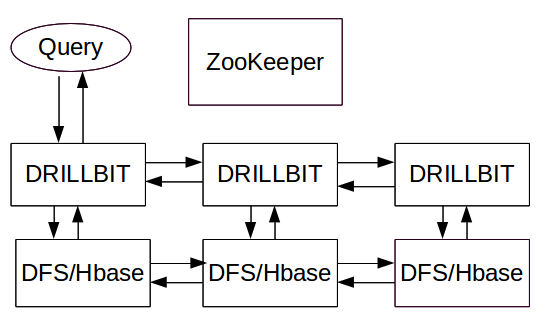
\includegraphics[width=\linewidth]{images/Architecture.png}}
		\caption{Query Execution Workflow.}
		\label{fig:Drill-arch}
	\end{figure}
	
	Figure 1. above describes the basic query execution workflow.Important thing to notice here is that each of the Drillbits are equal and there is no Master-Slave concept. So, the request from the client can go to any of of the drillbit depending upon its availability. It is also a completely scalable architecture that allows to add in more drillbits as and when
	required\cite{Query-Execution}.

\subsection{Columnar Execution}
	Drill is Columnar in storage as well as memory. It means that it does not have
	to materialize the data into row format and can perform all SQL operations like
	join, sorting, etc directly on columnar data  without having to change the data.
	The benefit of this is that it not only boosts the performance but also saves
	the memory footprint that Drill has to occupy during query execution.

\subsection{Vectorized Processing}
	Drill  provides a vectorized execution engine to offer high memory and CPU
	efficiencies along with rapid performance for a wide variety of analytic
	queries. Instead of working on single records at any given time, Drill allows
	CPU to work on vectors, which are arrays of values from many different set of
	records in table. So, Drill works on more than one record at a time to achieve
	efficiency.

\subsection*{Optimistic/In-Memory}
	Drill is very optimistic in the sense it assumes that the chances of failure
	like hardware or node failure is very uncommon during the short execution of the
	query.So, it tries to execute as much as possible in memory without writing
	anything to disk for checkpoint and recovery purposes. Drill uses the
	traditional Pipe-line execution model in which all the tasks are executed in
	parallel and in different stages in different parts of the cluster.This enables
	Drill to achieve high speed performance in seconds.

\subsection{Datastores Support}
	Drill is build for non-relation datastores like Hadoop, NoSQL, and cloud
	storage.
	Currently following datastores are supported:
	
	\begin{itemize}
		\item \textbf{Hadoop}: All Hadoop distributions (HDFS API 2.3+), including
		Apache Hadoop, MapR, CDH and Amazon EMRfor Data Ingestion
		\item \textbf{NoSQL}: MongoDB, HBase
		\item \textbf{Cloud storage}: Amazon S3, Google Cloud Storage, Azure Blog
		Storage, Swift
		
	\end{itemize}

\subsection{Client Support}
	Drill currently supports following clients:
	
	\begin{itemize}
		\item \textbf{BI tools} via the ODBC and JDBC drivers (eg, Tableau, Excel,
		MicroStrategy, Spotfire, QlikView, Business Objects)
		\item \textbf{Custom applications} via the REST API
		\item \textbf{Java and C applications} via the dedicated Java and C libraries
		
	\end{itemize}

\section{Comparison}
	Drill supports various non-relational datastores including Hadoop. However,
	Drill takes a different approach compared to popular SQL-on-Hadoop technologies
	like Hive and Impala. For example, it lets users directly query self-describing
	data (eg, JSON) without having to create and manage schemas.Moreover, Hive is a
	typical batch processing framework best suitable for long-running jobs, Drill on
	the other hand is suitable for short-running jobs like data exploration and BI.
	Unlike Hive, Drill is not limited to Hadoop. Drill can also query NoSQL
	databases (eg, MongoDB, HBase) and cloud storage (eg, Amazon S3, Google Cloud
	Storage, Azure Blob Storage, Swift).

\section{Getting started}
	Step-by-step procedures to download, install and get started with Drill can be found on-line.\cite{Tutorial}

\section{Conclusion}
	Apache Drill allows us to use familiar querying language (SQL) against different
	data sources.It provides a single SQL interface for self service data
	exploration for structured and semi-structured data Source without any IT
	intervention. Drill also allows us to use familiar BI tools like Tableau and
	Excel for data exploration without any time-consuming/expensive programing and
	data definition. Apache Drill is making big data analytics more accessible to
	wider groups of people. 

\section*{Acknowledgements}

	The author thanks Prof. Gregor von Laszewski for his technical guidance.

% Bibliography

\bibliography{references}

\end{document}
